\chapter{Evaluación de la Solución}

A continuación se describe el proceso de evaluación realizado, los resultados
obtenidos y los aspectos de mejora de la aplicación.

\section{Proceso de Evaluación}

El proceso de evaluación del software se enfocó principalmente en determinar la
correctitud de operaciones realizadas por el sistema, y la adherencia de éste al
flujo de trabajo definido para cada uno de los participantes. Para las pruebas
el software se dejó disponible en el siguiente URL:
https://postulaciones.netlify.app/. Se ingresaron 17 postulaciones al sistema,
todas ellas con información ficticia, por razones de privacidad.

Además se definieron tres usuarios con perfil de \emph{asistente}, cuatro con perfil de
\emph{evaluador} (miembros del comité académico del programa) y un coordinador. La
evaluación fue hecha por los actuales coordinadores del Programa, quienes
asumieron temporalmente los distintos roles (perfiles de usuario) para llevar
adelante el proceso completo. Es importante destacar que estas personas han
participado en la evaluación de postulaciones durante al menos los últimos 10
años. 

Los distintos usuarios se autenticaron en la aplicación, y realizaron su labor
habitual utilizando el nuevo sistema. Particularmente, durante esta evaluación
los asistentes procesaron 12 de las 14 postulaciones disponibles. Los
evaluadores revisaron y emitieron un juicio sobre 11 de ellas, y el coordinador
decidió la aceptación o rechazo de sobre 6 postulaciones. Esto significa que se
realizó el flujo de trabajo completo para 6 postulaciones, involucrando a todos
los actores en el proceso. Además, se realizó una parte del flujo de trabajo
para otras 6 postulaciones.

El estado en que quedaron las postulaciones se muestra en la siguiente figura,
donde el estado “\emph{pendiente}” significa que el asistente aún no ha revisado
la postulación, y por lo tanto, no es posible evaluarla. El estado
“\emph{resuelta}”indica que los evaluadores emitieron su opinión, y el
coordinador resolvió en base a ellas. El estado “\emph{en evaluación por el
comité académico}” significa que la postulación está siendo evaluada, y que al
menos un miembro de dicho comité no ha emitido su opinión respecto a la
aceptación o rechazo de la misma. Finalmente, el estado “\emph{esperando
resolución}” significa que todos los miembros del comité académico han emitido
su opinión, y sólo resta que el coordinador decida y registre la decisión en
UCampus.

\begin{figure}[!ht]
    \begin{center}
        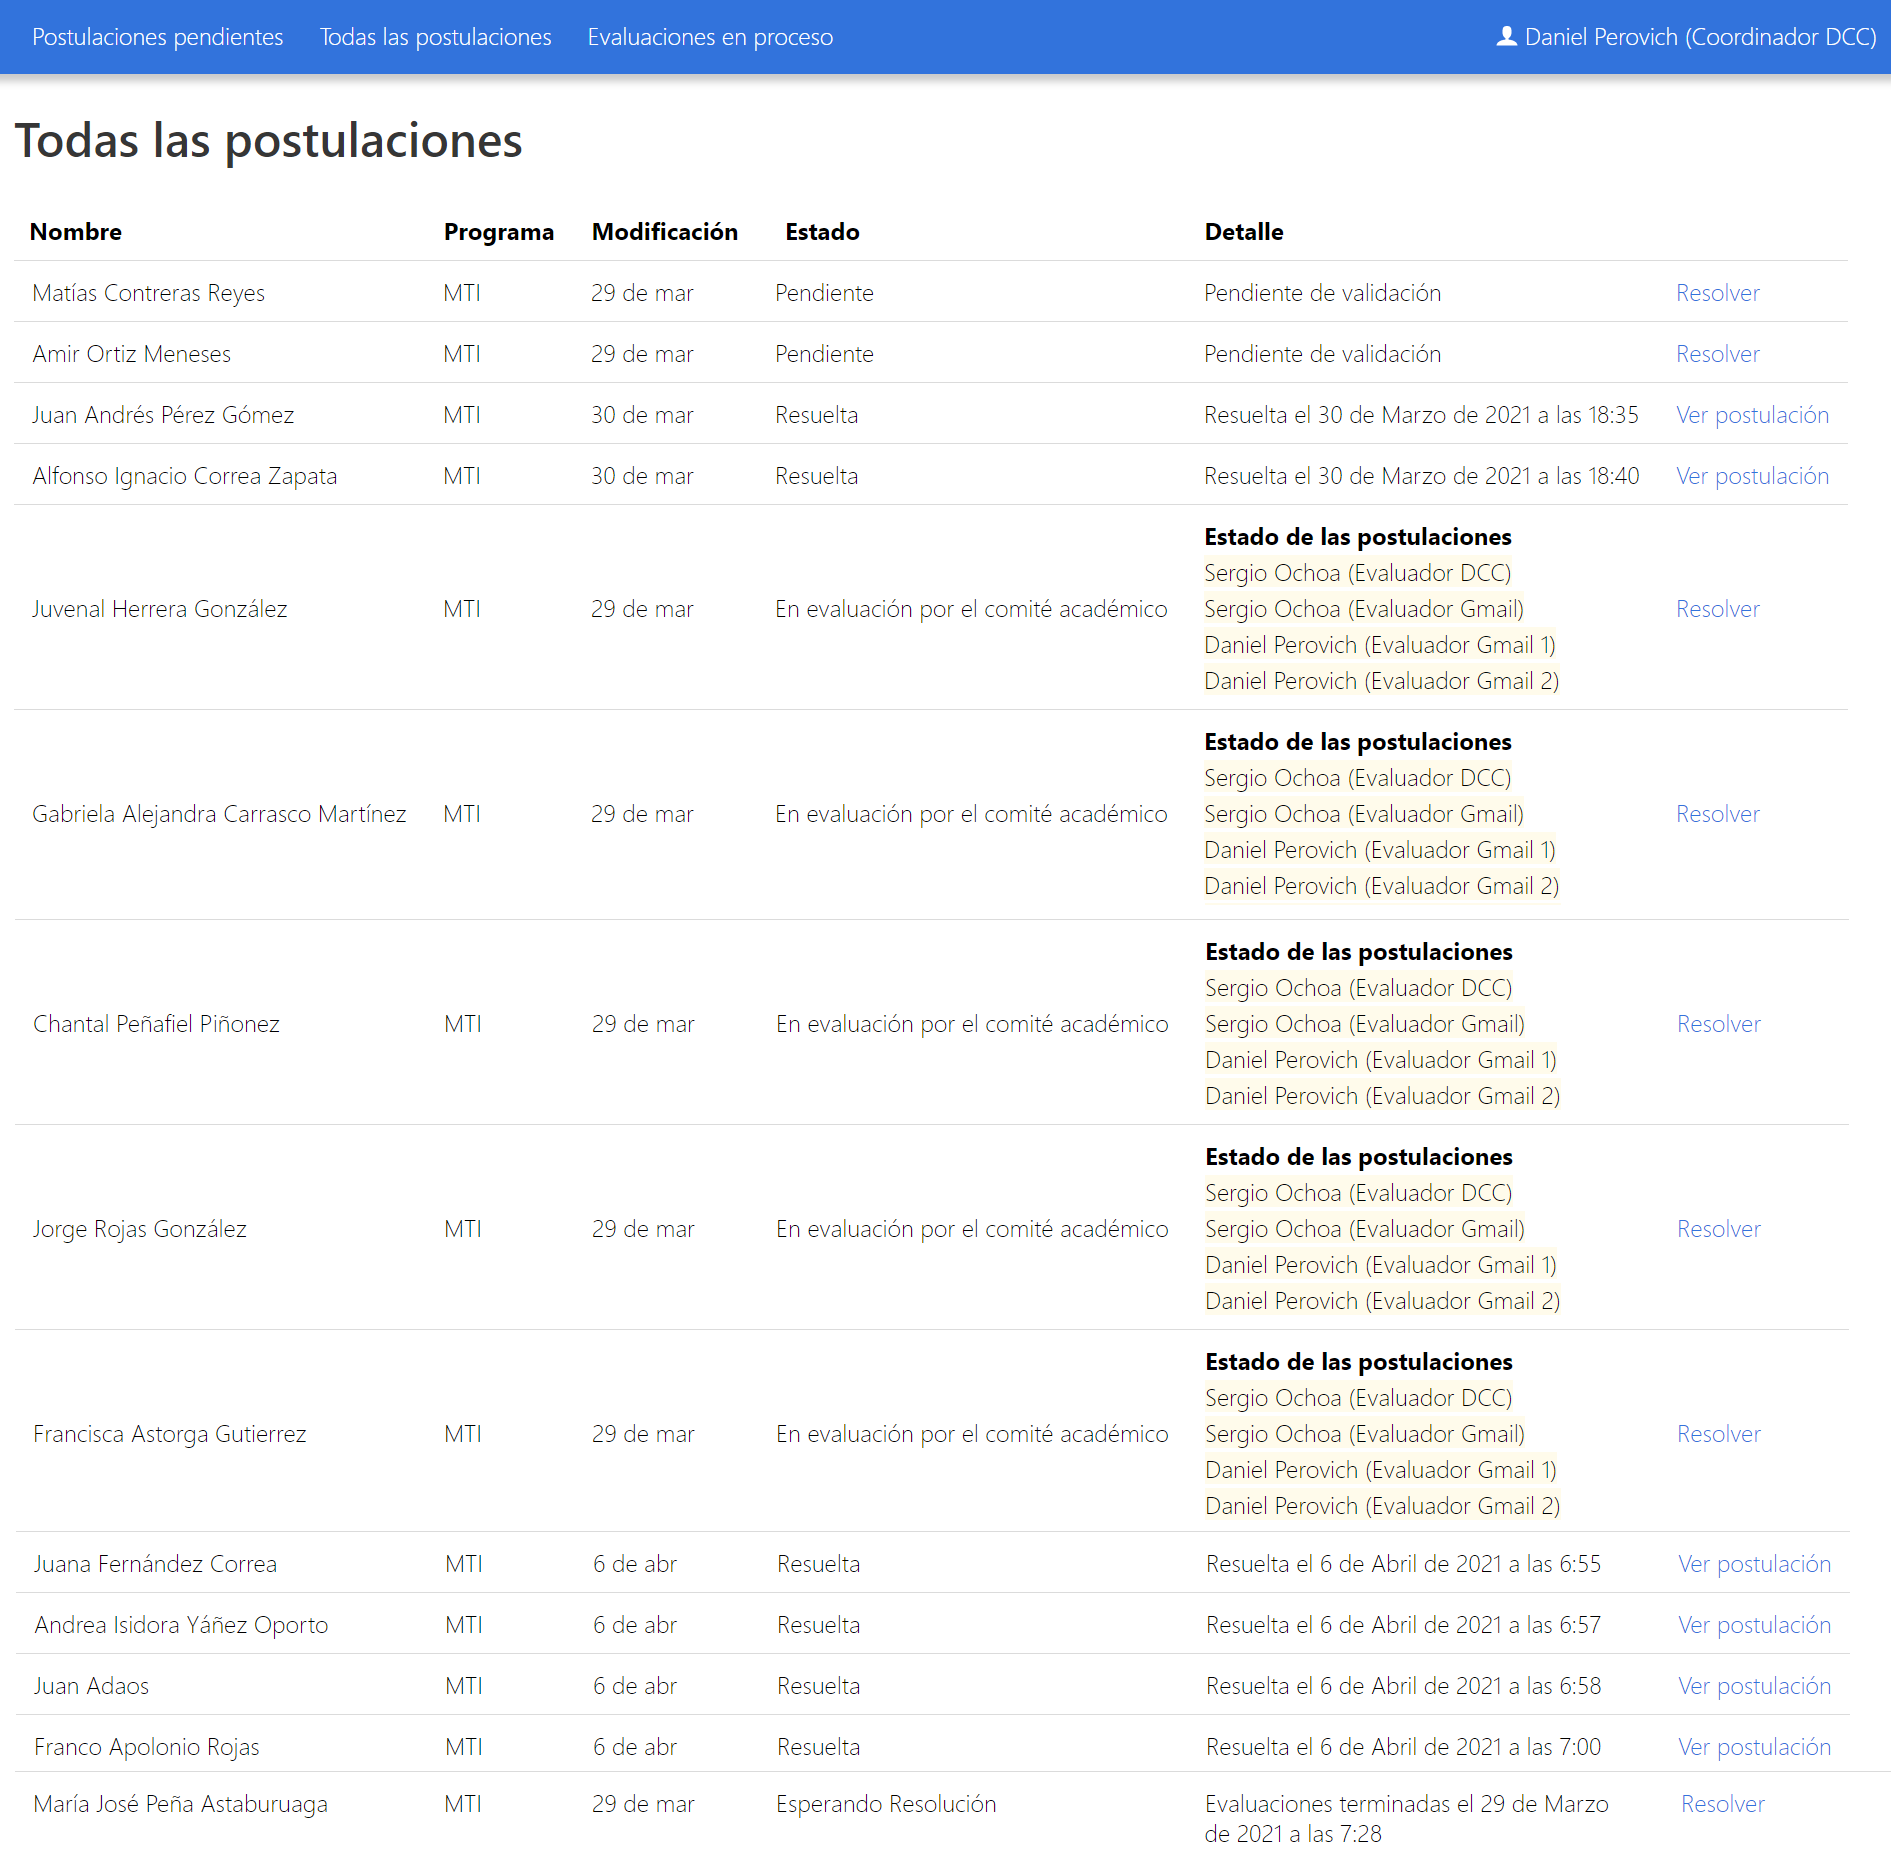
\includegraphics[scale=0.23]{imagenes/05-estado-final-evaluaciones.png}
    \end{center}
    \caption{Formulario de resolución de postulaciones}
    \label{fig:estado-final-evaluaciones}
\end{figure}

\section{Sobre los resultados obtenidos}

En primer lugar es importante destacar que la aplicación logró dar soporte al
workflow completo del proceso de evaluación, considerando los roles de los
participantes, y sin ningún error de lógica. Tampoco se detectó inestabilidad
del sistema, y su usabilidad fue calificada como “buena” por parte de los
usuarios. En ese sentido se puede afirmar que se alcanzaron los objetivos
definidos en esta memoria, y que la aplicación resultante está en condiciones de
probarse en marcha blanca con postulaciones reales.

Por otra parte, los usuarios hicieron varios comentarios orientados a mejorar
las interfaces del sistema, en pos de facilitar el trabajo de cada rol. También
observaron varios aspectos que restringen la información a la que pueden acceder
algunos roles, respecto de las postulaciones. A continuación se indican los más
importantes:

\begin{itemize}
    \item Que las tablas que muestran las postulaciones en los diferentes tracks
    permitan ordenar dichas postulaciones por columna, para así hacer más
    flexible y simple la identificación de postulaciones en diferentes estados,
    o bien identificar postulaciones en particular.
    \item Que los asistentes no puedan ver las evaluaciones hechas por los
    miembros del comité académico. Esto incluye la resolución propuesta y los
    comentarios realizados para cada uno de los ítems de evaluación. En resumen,
    los asistentes sólo podrán ver ver que la evaluación fue hecha por un
    evaluador un cierto día y hora.
    \item Un evaluador solo debe poder ver las postulaciones en las que
    participó como evaluador (independientemente de si realizó la evaluación, o
    se la cancelaron). Este tipo de usuario no debe poder ver las postulaciones
    en las que no participó. 
    \item Reemplazar las actuales tres opciones de menú, por las que se indican
    a continuación, solo por una cuestión de facilidad de comprensión y acceso a
    las postulaciones por parte de los diferentes usuarios:
    \begin{itemize}
        \item \emph{Postulaciones abiertas}. Mostrar todas las postulaciones que
        aún tienen tareas pendientes de ser realizadas, ordenadas de más
        antiguas a más nuevas por fecha de postulación.
        \item \emph{Postulaciones cerradas}. Mostrar todas las postulaciones que
        ya fueron resueltas (ya sea aceptadas o rechazadas), ordenadas de más
        nueva a más antiguas por fecha de postulación. usuario tiene asignadas
        para evaluar, ordenadas de más antiguas a más nuevas por fecha límite
        para hacer la evaluación.
        \item \emph{Evaluaciones pendientes}. Mostrar todas las postulaciones
        que el usuario tiene asignadas para evaluar, ordenadas de más antiguas a
        más nuevas por fecha límite para hacer la evaluación.
        \item \emph{Evaluaciones realizadas}. Mostrar todas las postulaciones que el
        usuario ya evaluó, ordenadas de más nueva a más antiguas por fecha en
        que fue realizada la evaluación.
    \end{itemize}
\end{itemize}

Es importante destacar que estos ajustes al sistema plantean reorganizar o
limitar el acceso a los servicios que ya están implementados. Por lo tanto, su
incorporación no significa un gran desafío para el proyecto, y son fácilmente
realizables.

